\documentclass[11pt, a4]{article}
\usepackage{geometry}
\geometry{margin=1.25in}
\usepackage[utf8]{inputenc}
\usepackage[english]{babel}
\usepackage{amsmath}
\usepackage{graphicx}
\graphicspath{ {../figures/} }
\usepackage{placeins}
\usepackage{booktabs}

\title{Supermarket sales \\
		\large Exploratory Data Analysis for Machine Learning - Course Project}
\author{Caio Mescouto Terra de Souza}
\date{\today}

\begin{document}

\maketitle

\section*{Brief Description of the Data Set and a Summary of its Attributes}

Supermarket sales data set \cite{sales} is a historical record of sales data in 3 different Branches for 3 months. Each observation has 17 features that indicates where the purchase happen (Branch, City), when (Date and Time), the Product Line, Unit Price, Quantity, Payment method, Cost of goods sold, margins, Taxes and Customer informations (Gender and Type) in addition to stratification rating on their overall shopping experience.

The data set has 1000 observations and no missing values. The variables are presented below (data dictionary and types of attributes):

- \textbf{Invoice id} (categorical - object): Computer generated sales slip invoice identification number

- \textbf{Branch} (categorical - object): Branch of supercenter (3 branches are available identified by A, B and C).

- \textbf{City} (categorical - object): Location of supercenters

- \textbf{Customer type} (Categorical - object): Type of customers, recorded by Members for customers using member card and Normal for without member card.

- \textbf{Gender} (categorical - object): Gender type of customer

- \textbf{Product line} (Categorical - object): General item categorization groups - Electronic accessories, Fashion accessories, Food and beverages, Health and beauty, Home and lifestyle, Sports and travel

- \textbf{Unit price} (numerical - float64): Price of each product in \$

- \textbf{Quantity} (numerical - int64): Number of products purchased by customer

- \textbf{Tax} (numerical - float64): 5\% tax fee for customer buying

- \textbf{Total} (numerical - float64): Total price including tax

- \textbf{Date} (categorical - object): Date of purchase (Record available from January 2019 to March 2019)

- \textbf{Time} (categorical - object): Purchase time (10am to 9pm)

- \textbf{Payment} (numerical - float64): Payment used by customer for purchase (3 methods are available – Cash, Credit card and Ewallet)

- \textbf{COGS} (numerical - float64): Cost of goods sold

- \textbf{Gross margin percentage} (numerical - float64): Gross margin percentage

- \textbf{Gross income} (numerical - float64): Gross income

- \textbf{Rating} (numerical - float64): Customer stratification rating on their overall shopping experience (On a scale of 1 to 10)




\section*{Initial Plan for Data Exploration}

At a first glimpse on the data set we found some constraints that will guide the plan for Data Exploration.

\textbf{Main constraints:}
\begin{itemize}
\item Branch and City is the same information, meaning that we have only one information about geographical position;
\item Tax and gross margin have no variance, meaning that all product lines have the same tax and gross margin, so all analysis based on Cost of Goods, Income, Margins and Taxes are meaningless;
\item The record available has only 3 months of data, so the seasonality that can be explored are just day of the week and hour of the day.
\end{itemize}

Considering the restrictions presented above, the \textbf{promising starting points} for exploratory data analysis are highlighted below. These starting points were thought as actionable tasks that can improve the company result.
\begin{itemize}
\item Does the rating differ between branches? If so, what hypotheses can explain and guide a solution?
\item Do branches have different mean tickets? If so, why?
\item Does the mean ticket differ between day of the week or hour?
\item Does the rating differ between day of the week or hour?
\end{itemize}

Finally, the \textbf{Roadmap for exploring the data} is:

\begin{itemize}
\item Data cleaning: drop all meaningless variables and looking for outliers that can problematic attributes;
\item Data transformation: At the first moment only Date and Time will be merged;
\item Data exploration: Get to know the numerical variables distributions and highlight the transformations needed. Get to know the categorical variables, the number of categories in each one and if it can be meaningful;
\item Correlations: The next step is to analyse the correlations between numerical variables before the feature engineering process;
\item Feature Engineering;
\item Draw the insights and hypotheses;
\item Test the most promising hypothesis;
\item Suggest next steps for further investigations according with was highlighted during the exploration;
\item Final comments and conclusions.

\end{itemize}


 

\section*{Data Cleaning and Feature Engineering}

\subsection*{Data Cleaning}

The data set does not have missing data or outliers that could indicate problematic attributes or observation. As stated before some attributes were dropped and Date and Time was merged as timestamps. After the data cleaning process the data set has the following attributes (Table \ref{table:1})

DatetimeIndex: 1000 entries, 2019-01-05 13:08:00 to 2019-02-18 13:28:00
\begin{table}[h!]
\centering
\begin{tabular}{l c c}
\toprule
\textbf{Column} & \textbf{Dtype} & \textbf{Total var. or range} \\
\midrule
Branch & object & 3\\
Customer type & object & 2\\
Gender & object & 2\\
Product line & object & 6 \\ 
Unit price & float64 &10.08 - 99.96 \\
Quantity & int64  &1 - 10\\
Total & float64 &10.68 - 1042.65\\
Payment & object &3\\
Rating & float64 &4 - 10\\
\bottomrule
\end{tabular}
\caption{Data Set Attributes}
\label{table:1}
\end{table}


\subsection*{Feature Engineering}

First of all, as we are mainly interested in the differences between branches, we observed that the distribution between them is almost a third part each, and the same behavior is observed for all categorical attributes. Besides that, as presented before, the number of variables of each attribute is small. In addition neither of them are ranked, meaning that all are good candidates for One Hot Encoding as feature engineering for machine learning preprocessing.

Considering the numerical attributes, only a few transformations seem worth it. “Total” is the total invoice price and it is clearly right skewed (Figure \ref{fig:hist}) and a log transformation is a good way to better fit the variable for machine learning algorithms. The rest of the numerical variables are equally distributed, so only a standardization is required to improve the fit in the models. 

\begin{figure}[!h]
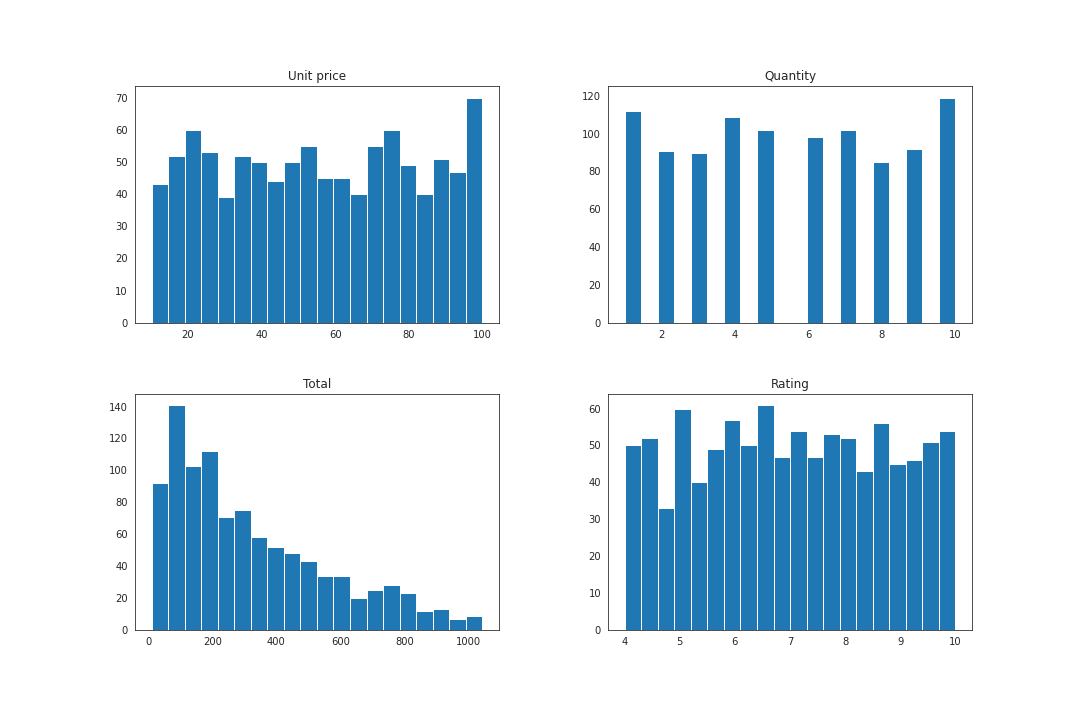
\includegraphics[]{hist}
\centering
\caption{Histograms per Branches}
\label{fig:hist}
\end{figure}

\section*{Key Findings and Insights}

Besides the \textit{Tota}l distribution (Figure \ref{fig:hist}) per branches that present a similar behavior, the mean and the median are higher in \textit{C} followed by \textit{B} and \textit{A} (Table \ref{table:2}). This difference is most explained by the \textit{Unit price} of the products as de mean and median quantity are fairly the same through the branches. However, these differences do not seem significant as the standard deviation is very high.


\begin{table}[h!]
\centering
\begin{tabular}{l c c c}
\toprule
\textbf{Statistic} & \textbf{A} & \textbf{B} & \textbf{C} \\
\midrule
mean &	312.35& 	319.87& 	337.10\\
median& 	240.83& 	252.88& 	271.42\\
std 	&231.64 	&242.45& 	263.16\\
\bottomrule
\end{tabular}
\caption{Total per Branches}
\label{table:2}
\end{table}

There is no correlation between \textit{Total} and \textit{Rating} neither in all data sets nor by branches, as the \textit{A} and \textit{B} are similarly rated and the \textit{B} has the lowest \textit{Rating} between them (Figure \ref{fig:rating}). Again the significance seems not large enough, but these first findings are good guides for the next steps. 

\begin{figure}[!h]
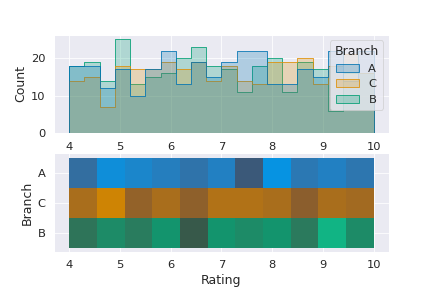
\includegraphics[]{rating}
\centering
\caption{Ratings per Branches}
\label{fig:rating}
\end{figure}

\begin{figure}[!h]
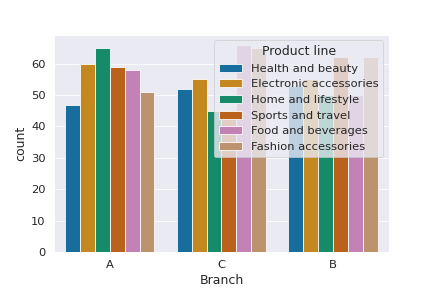
\includegraphics[]{branch_line}
\centering
\caption{Product lines per Branches}
\label{fig:prodb}
\end{figure}

\begin{figure}[!h]
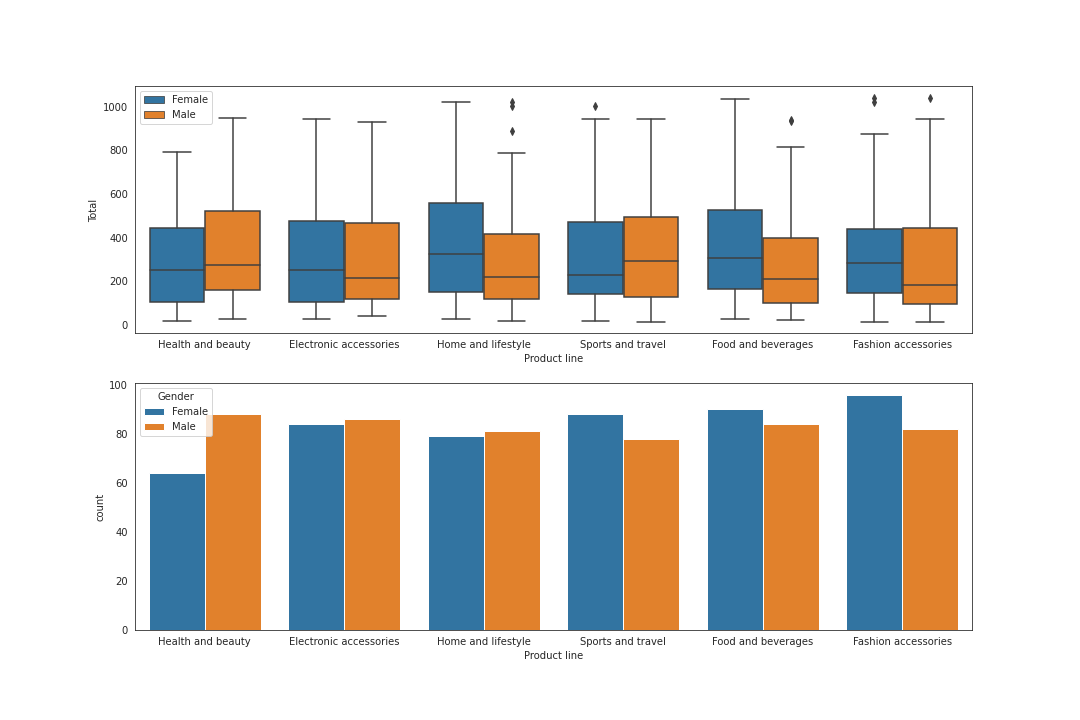
\includegraphics[]{boxgender}
\centering
\caption{Boxplot Product line per Gender}
\label{fig:bgedner}
\end{figure}

Analyzing\textit{Branch} per \textit{Gender} was observed that \textit{A} has more men invoices and \textit{C} women ones. We also know that \textit{Female} spend more than \textit{Male}, knowing that this relationship of invoice price is the same for \textit{Branch}, this is meaningful, but we cannot explain causation. In addition, we also observed that Membership and payment method follow same distributions. In brief \textbf{\textit{Female} are majority among customer members and use more with \textit{Cash}, the same relationship was observed for \textit{C}. \textit{Male} are the majority among normal customers and use more \textit{Ewallet}.}


The exploration of the \textit{Product line} brought interesting insights because we can observe variance between \textit{Product line} and \textit{Branch} (Figure \ref{fig:prodb}) and \textit{Gender} (Figure \ref{fig:bgedner}). First of all \textbf{Women are the major buyers of \textit{Sports and travel}}, but \textit{C}, where they are the majority of clients performs badly in this line. however, looking further the reality is that, \textbf{this \textit{Branch} performs badly with men in this line, in quantity of invoices and average ticket compare others.} But as the rating is high (Table \ref{table:3}), one hypothesis is that this \textit{Branch} doesn’t have more expensive products for men. We need to investigate further to confirm this hypothesis, but a suggested action could be to expand the range of these products in this \textit{Branch}. 

\begin{table}[h!]
\centering
\begin{tabular}{l c c c c}
\toprule
\textbf{Branch} & \textbf{Gender} & \textbf{Count} & \textbf{Mean}&\textbf{Rating} \\
\midrule
A&  Female& 	29& 279.83	&7.16 	\\
&Male 	&30 	&375.25 &7.35 	\\
B& 	Female& 	30& 	307.09 &	6.37	\\
&Male 	&32 &	336.73	&6.64 	\\
C& 	Female& 	29& 	387.82 	&	6.79\\	
&Male 	&16 	&282.20&  	7.47 \\
\bottomrule
\end{tabular}
\caption{Sports and travel per Branch and Gender}
\label{table:3}
\end{table}

The second insight is \textbf{\textit{Male} are the major buyer of \textit{Health and beauty}}, but they buy more in \textit{B} and \textit{C} and with high ticket, even if they are the majority of clients in \textit{A}.	The same hyphotesis and suggestion presented before is applied here (Table \ref{table:4}).

\begin{table}[h!]
\centering
\begin{tabular}{l c c c}
\toprule
\textbf{Branch} & \textbf{Gender} & \textbf{Count} & \textbf{Mean} \\
\midrule
A &	Female& 	21& 	272.14\\
&Male 	&26 	&264.73\\
B& 	Female& 	20& 	320.02\\
&Male 	&33 	&411.52\\
C &	Female& 	23& 	280.25\\
&Male 	&29& 	350.68	\\
\bottomrule
\end{tabular}
\caption{Health and beauty per Branch and Gender}
\label{table:4}
\end{table}

The third insight is that \textbf{men buy less \textit{Fashion} articles in \textit{A} than \textit{C} and the rating is also higher in \textit{C} and this is also true for women.} It would be related to the quality of the products in \textit{A}.

\begin{table}[h!]
\centering
\begin{tabular}{l c c c}
\toprule
\textbf{Branch} & \textbf{Count} & \textbf{Rating} \\
\midrule
A& 	51 	&6.88\\
C &	65 	&7.44\\
\bottomrule
\end{tabular}
\caption{Health and beauty per Branch and Gender}
\label{table:4}
\end{table}

Finally, we can infer women spend more in \textit{Food and Bevarage} and \textit{Home and Lifestyle} because usually they are responsible for maintaining the home, and men spend more in \textit{Health and beauty} because they use more popular products that are found in supermarkets.

Moving on the seasonality aspect, we can observe daily variation in all branches, however, \textit{A} seems less extreme (Figure \ref{fig:season}). In fact, \textit{A} seems more stable than \textit{B} (Figure \ref{fig:week}). In addition, we also analyze seasonality per hour(Figure \ref{fig:hour}. \textbf{\textit{B} has a high traffic at 13h and 19h during working days} .We also noticed that the movement is high on Saturdays and is the branch that sells the most products in \textit{Sports and Travel}. It can indicate that it is close to workplaces and people go there after work or at lunch to buy a few things, but they also have a good line of \textit{Sport and Travel}, which motivates customers to move around on Saturdays .

\begin{figure}[!h]
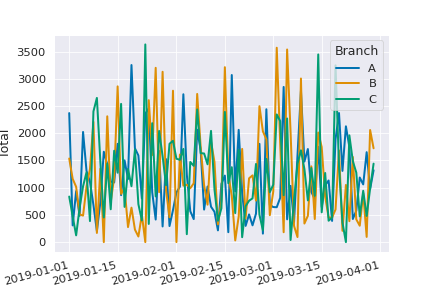
\includegraphics[scale=0.8]{season}
\centering
\caption{Sum of Total per Day}
\label{fig:season}
\end{figure}

\begin{figure}[!h]
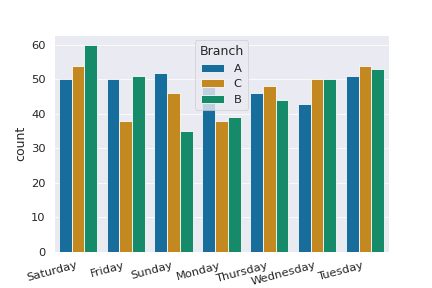
\includegraphics[scale=0.8]{week}
\centering
\caption{Invoices per day of the week}
\label{fig:week}
\end{figure}

\begin{figure}[!h]
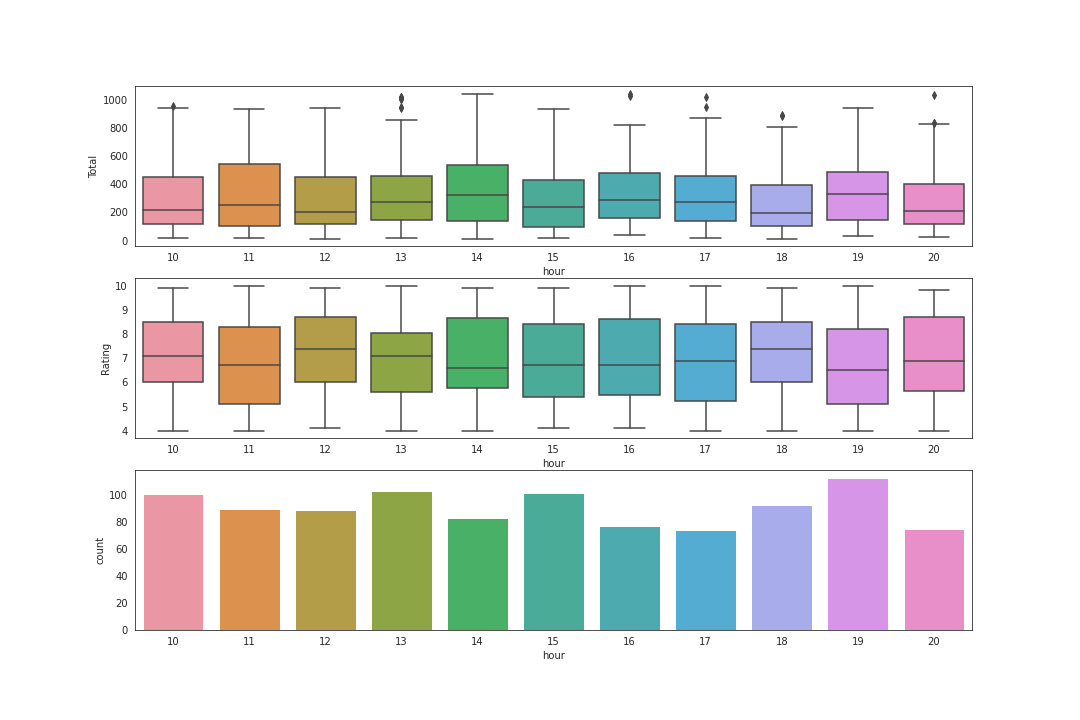
\includegraphics[scale=0.8]{hour}
\centering
\caption{Invoices per hours (working days)}
\label{fig:hour}
\end{figure}


\section*{Main Hypotheses}

Considering the insights presented in the preceding section, we can sintetize some hypotheses.

\begin{itemize}
\item Considering \textit{Sport and Travel}, male invoices in \textit{C} are significantly lower than invoices in \textit{A};\\
\item Men are more satisfied buying \textit{Fashion accessories} in \textit{C} than in \textit{A};\\
\item \textit{B} sells more during working days at lunch time (13:00) and 19:00 than \textit{A} and \textit{C}. 
\end{itemize}

\section*{Significance Test}

To test one of those hypotheses, a formal significance test was carried out for the third hypothesis raised. As the distributions are not normal, but have similar shape (Figure \ref{fig:test}), the \textit{Mann-Whitney} non-parametric test was applied and the result is presented below. 

\begin{figure}
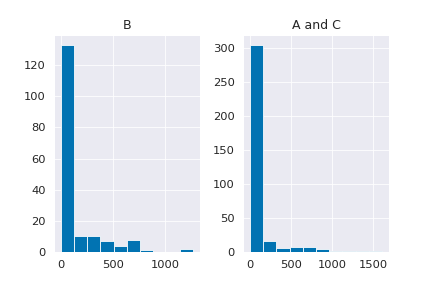
\includegraphics[]{test}
\centering
\caption{Total histogram}
\label{fig:test}
\end{figure}

\begin{align*}
&\alpha = 0.05\\
&H_0: \text{The sum of Total during working days and during 13:00 and 19:00 is the same at all three Branch}  \\
&H_1:\text{\textit{B} sells more during working days at lunch time (13:00) and 19:00 than \textit{A} and \textit{C}.}\\
& p-value=0.01 < \alpha\\
& statistic=28009.0\\
\end{align*}

As the $p-value$ is smaller than $\alpha$, the null hypothesis can be rejected.

\section*{Next Steps}

Seasonalities can be a good topic to investigate more, the relationship with ratings on days of the week and hours can indicate some issues, for example few employees helping customers during rush hours, or a specific employee group that are not well trained in customer assistance.

Other interesting topic is the \textit{Product line}, as we found some differences between \textit{Gender} and \textit{Branch} that can indicate the necessity of adjust in some lines depending on the \textit{Branch}. 

\section*{Coments About the Data Set}

The data set has a time constraint for example for forecasting demand, another problem is the level of information related to products, only the big lines are available and further investigations on consumptions are impossible. In addition, Customer ID can help with suggestion algorithms. Finally, the information about Tax and Cost are meaningless and any analysis on costs and earnings is impossible from this data set. 

\FloatBarrier

\begin{thebibliography}{9}

\bibitem{sales} 
Supermarket sales:
Historical record of sales data in 3 different supermarkets,
\\\texttt{https://www.kaggle.com/aungpyaeap/supermarket-sales}
\end{thebibliography}

\end{document}